\scanpage{58}
la formule ci-dessus;
\deleted{\unsure{Il ne semble plus} \unsure{possible que}}
\inserted{À priori}, la cohomologie stratifiante d'un Module stratifié s'explicite comme une hypercohomologie zariskienne (et encore, dans un complexe dont la \deleted{\unsure{d}} différentielle n'est pas linéaire!), \deleted{et} mais l'inverse ne semble pas vrai.

On va voir pourtant que, dans un certain sens, il en est bien ainsi.
À peu de choses près, on associe à tt Module quasi-cohérent $\mathcal{F}$ (\uline{sans stratification}) un Module \deleted{quasi-cohérent} \inserted{(plutôt un pro-Module pro-quasi-cohérent)} $Q^0(\mathcal{F})$ stratifié, dont la cohomologie stratifiante est la coh. zariskienne \uline{ordinaire} de $X$.
De plus, $Q^0(\mathcal{F})$ est un foncteur en $\mathcal{F}$, non \unsure{seulement} pour des hom linéaires $\mathcal{F}\to\mathcal{G}$, mais $\overline{\mathrm m}$ \deleted{\unsure{pour} \illegible{1}} \inserted{(comme} faisceau \deleted{additif, $\overline{\mathrm m}$ de} d'$\mathcal{O}_X$-modules) pour des $\uline{D}:\mathcal{F}\unsure{\mathbin{-}|\to}\mathcal{G}$ qui sont seulement des op. diff. rel/$S$.
\margin{\figure{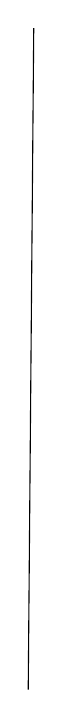
\begin{tikzpicture}
\draw (0,0)--(-0.07,-8.4);
\end{tikzpicture}}}
\deleted{\unsure{Il faut} \illegible{4}}
[Dans le cas très particulier où $\operatorname{diag}_{X/S}:X\longrightarrow X\times_S X$ est une immersion \unsure{nilpotente}, donc \deleted{\unsure{can.} $Q^0($} stratification /$S$ = donnée de descente à $S$, $Q^0(\mathcal{F})=f^*f_*(\mathcal{F})$].

L'intérêt \inserted{de ces divers points} est que \uline{l'hypercoh.} \inserted{zariskienne ordinaire} d'un complexe d'op. diff. \uline{peut s'interpréter comme la coh. stratifiante du complexe} correspondant de faisceaux stratifiés...!

\margin{57}
